\documentclass[10pt,a4paper,twocolumn]{article}

% ─── core packages ──────────────────────────────────────────────────────────
\usepackage[utf8]{inputenc}
\usepackage[T1]{fontenc}
\usepackage{textcomp}
\usepackage{amsmath,amssymb,graphicx,hyperref,microtype,enumitem}
\usepackage{xcolor}
\usepackage{listings}
\usepackage{geometry}
  \geometry{margin=0.7in,columnsep=0.3in}
\usepackage{balance}
\usepackage{dblfloatfix}
\usepackage{needspace}
\usepackage{tikz}
  \usetikzlibrary{matrix,positioning,arrows.meta,shapes,calc}
\usepackage{commath}
\usepackage{pgfplots}
  \pgfplotsset{compat=1.18}
\usepackage{subcaption}
\usepackage{etoolbox}

% ─── version label (left margin) ────────────────────────────────────────────
\usepackage{eso-pic}
\immediate\write18{git rev-parse --short HEAD > \jobname.githash}%
\newcommand\versionnumber{Git~%
  \IfFileExists{\jobname.githash}{\input{\jobname.githash}}{unknown}%
}
\AddToShipoutPictureBG*{%
  \AtPageUpperLeft{%
    \hspace*{1cm}% ← shift right by 1 cm; adjust as you like
    \raisebox{-0.5\paperheight}{%
      \rotatebox{90}{\color{gray!40}\small\versionnumber}%
    }%
  }%
}
% ─── listings setup ─────────────────────────────────────────────────────────
\BeforeBeginEnvironment{lstlisting}{%
  \par\noindent\begin{minipage}{\columnwidth}%
}
\AfterEndEnvironment{lstlisting}{%
  \end{minipage}\par\addvspace{\baselineskip}%
}

\lstdefinelanguage{Solidity}{
  keywords={function, contract, address, uint, uint256, bytes, bytes32, public,
            private, external, payable, view, pure, memory, storage, calldata,
            require, return, if, else, for, while, struct, mapping, emit, event,
            constructor, modifier, import, interface, using, library, new,
            delete, try, catch, revert, throw, this, super, virtual, override},
  keywordstyle=\color{blue}\bfseries,
  identifierstyle=\color{black},
  comment=[l]{//},
  morecomment=[s]{/*}{*/},
  commentstyle=\ttfamily\color{gray},
  stringstyle=\ttfamily\color{red},
  morestring=[b]', morestring=[b]"
}

\lstset{
  basicstyle=\ttfamily\scriptsize,
  breaklines=true,
  breakatwhitespace=true,
  postbreak=\mbox{\textcolor{red}{$\hookrightarrow$}\space},
  linewidth=\columnwidth,
  frame=single,
  numbers=left,
  numberstyle=\tiny,
  numbersep=5pt,
  captionpos=b,
  keepspaces=true,
  tabsize=2,
  showspaces=false,
  showstringspaces=false,
  showtabs=false
}

% ─── hyperlinks ─────────────────────────────────────────────────────────────
\hypersetup{colorlinks=true,linkcolor=blue,filecolor=magenta,urlcolor=blue}

% ─── document meta ──────────────────────────────────────────────────────────
\title{Holograph 2.0: Omnichain Token Launch \& Liquidity Automation\\[0.5em]
\large Implementing Protocol-Driven Deflationary Tokenomics}
\author{}
\date{}

\begin{document}
\maketitle

\section*{Abstract}
Holograph's initial iteration demonstrated the potential of identical-address omnichain tokens, establishing a new paradigm for crosschain asset deployment. Building on these foundations, the Holograph Protocol is being rebuilt with a leaner, trust-minimised architecture that leverages LayerZero V2's permissionless execution model. By embedding Doppler's Base/Unichain-native launch infrastructure and implementing HLG-centric tokenomics, the streamlined protocol ensures that every token launch and bridge transaction directly contributes to HLG deflation, creating a sustainable value engine anchored by intrinsic utility and ecosystem-driven demand. The result is a truly decentralised, capital-efficient omnichain standard that maintains perfect address sameness across all supported networks.

\section{Introduction \& Strategic Focus}
\subsection{Evolution of crosschain Interoperability}
The blockchain ecosystem has evolved from isolated layer-1 networks to an interconnected web of specialised chains, each with unique capabilities and trade-offs. However, this fragmentation has created significant challenges for developers and users alike, with assets scattered across multiple networks and crosschain transfers requiring cumbersome wrapping mechanisms that break composability and introduce trust assumptions.

Holograph was conceived to solve this foundational problem by enabling identical-address deployment of assets across multiple chains. This innovation maintains perfect composability and provenance without the need for wrapping or bridging artifacts that plague existing crosschain solutions.

\subsection{Core Differentiation}
Holograph's primary innovation lies in its ability to deploy tokens with mathematically guaranteed identical addresses across every supported chain. This capability enables:
\begin{itemize}
  \item True crosschain composability for smart contracts and dApps
  \item Simplified asset indexing and verification across networks
  \item Seamless interoperability for both ERC-20 tokens and NFTs
  \item Verifiable onchain provenance tracing regardless of origin chain
\end{itemize}

Unlike other crosschain protocols that rely on wrapping, mapping, or synthetic representations, Holograph's identical-address tokens represent the same asset regardless of which chain they exist on, preserving their fundamental properties and relationships across the entire ecosystem.

\subsection{Technical Advancements}
The Holograph reboot introduces several critical architecture improvements:
\begin{itemize}
  \item Transition from centralised operators to permissionless execution via LayerZero V2
  \item Integration with Doppler's proven Dutch-auction and dynamic bonding-curve mechanisms
  \item Implementation of a robust fee-capture system with automated HLG swap-and-burn
  \item Enhanced security through TWAP-guarded liquidity pools and circuit breakers
\end{itemize}

\subsection{Target Market Expansion}
While Holograph's initial implementation focused primarily on NFT applications, the protocol reboot significantly expands its utility to encompass:
\begin{itemize}
  \item Fungible-token (ERC-20) launches across multiple chains
  \item Real-world-asset (RWA) tokenisation with consistent addressing
  \item Crosschain governance and coordination systems
  \item DeFi protocols that benefit from atomic crosschain deployments
\end{itemize}

\section{Technical Architecture}

\subsection{System Architecture Diagram}
\begin{figure*}[t]
  \centering
  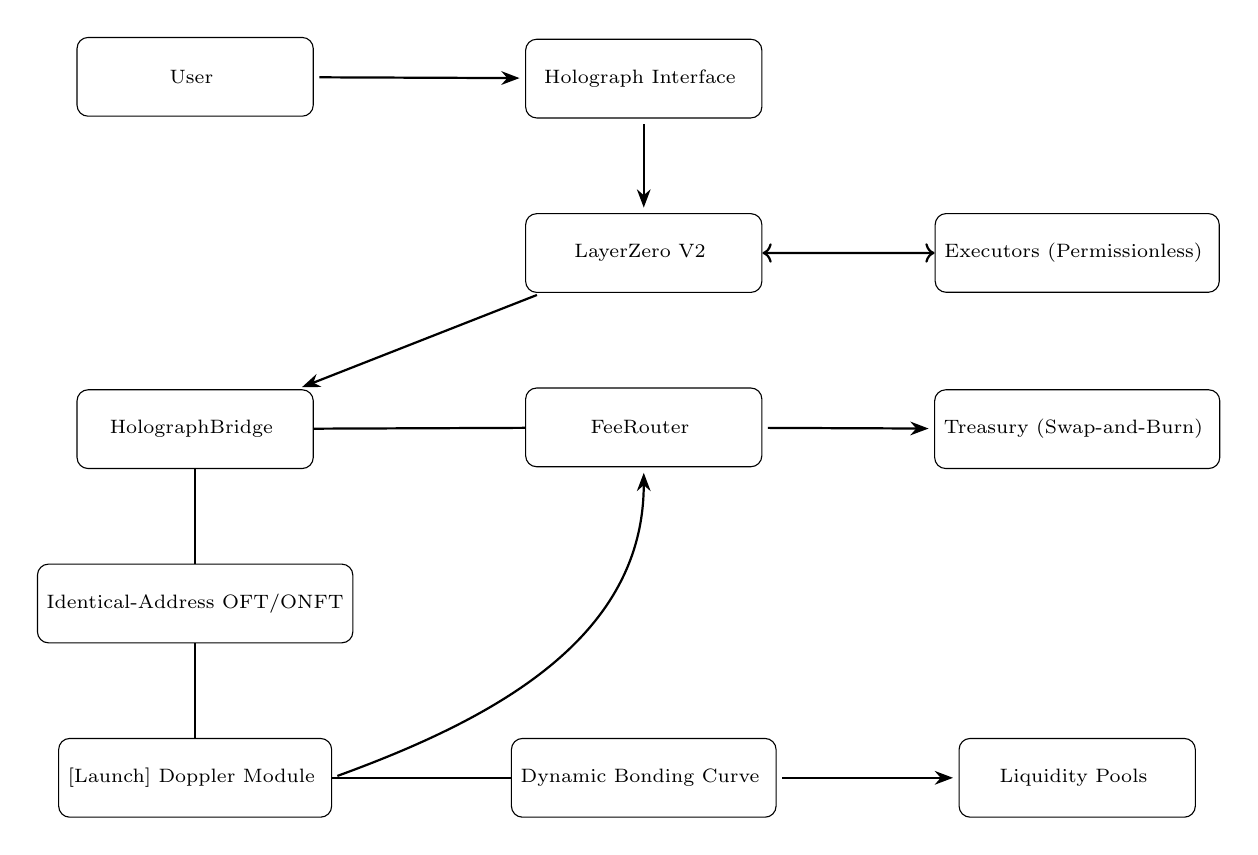
\begin{tikzpicture}[
    box/.style={
      draw,
      rounded corners=4pt,
      minimum width=3cm,
      minimum height=1cm,
      align=center,
      font=\scriptsize
    },
    arr/.style={
      -{Stealth},
      thick,
      shorten >=2pt,
      shorten <=2pt
    },
    row sep=1.2cm,
    column sep=2cm
  ]
    \matrix (M) [matrix of nodes, nodes=box] {
      User                      & Holograph Interface     &             \\
                               & [Bridge] LayerZero V2   & Executors (Permissionless)  \\
      HolographBridge           & FeeRouter               & Treasury (Swap-and-Burn)    \\
      Identical-Address OFT/ONFT&                         &             \\
      {}[Launch] Doppler Module & Dynamic Bonding Curve   & Liquidity Pools            \\
    };
    \draw[arr] (M-1-1) -- (M-1-2);
    \draw[arr] (M-1-2) -- (M-2-2);
    \draw[arr] (M-2-2) -- (M-3-1);
    \draw[arr] (M-3-1) -- (M-3-2) -- (M-3-3);
    \draw[arr] (M-3-1) -- (M-4-1) -- (M-5-1) -- (M-5-2) -- (M-5-3);
    \draw[<->,thick] (M-2-2) -- (M-2-3);
    \draw[arr]
      (M-5-1.east) to[out=20,in=-90] (M-3-2.south);
  \end{tikzpicture}
  \caption{Holograph 2.0 System Architecture}
  \label{fig:architecture}
\end{figure*}

\subsection{Core Components}

\subsubsection{LayerZero V2 Endpoint}
The LayerZero V2 Endpoint serves as the native onchain messaging interface for crosschain payload delivery. Each supported network has its own configured endpoint that handles message submission, gas abstraction, and proof verification hooks via Executors. This component represents a significant upgrade from the previous architecture, eliminating the need for trusted operators while maintaining security guarantees.

\subsubsection{Executors}
Executors are permissionless actors that finalize verified messages on destination chains. Any party can submit the Merkle or ZK-based proof published by LayerZero's Relayer Network and receive the gas tip. This removes the need for bonded operator pods, significantly reducing protocol costs while enhancing security through broader participation.

\subsubsection{HolographBridge}
The HolographBridge contract encodes and decodes omnichain fungible token (OFT) and omnichain non-fungible token (ONFT) transfers. In the updated architecture, the bridge connects to the LayerZeroModuleProxy for crosschain messaging. Upon message finalization, the \texttt{bridgeInRequest} function is invoked to mint or transfer assets as appropriate.

\Needspace*{5\baselineskip}
\begin{lstlisting}[language=Solidity, caption=HolographBridge.sol code snippet]
// In HolographBridge.sol
function bridgeOutRequest(...) external payable {
    // Encode mint payload for destination chains
    bytes memory payload = abi.encodeWithSelector(
        HolographERC20.mint.selector,
        recipient,
        amount
    );
    LayerZeroModule.sendPayload(targetChain, payload);
}
\end{lstlisting}

\subsubsection{FeeRouter}
The FeeRouter serves as the fee-routing hub for the protocol. It collects raw fees from HolographBridge operations, forwards 50\% to the Treasury for swap-and-burn operations, and routes the remainder to the StakingRewards contract to incentivize HLG staking.

\subsubsection{HolographTreasury}
The HolographTreasury contract functions as both fee sink and swap engine. It implements the swap-and-burn mechanism that automatically converts accumulated fees to HLG via Uniswap V4 with hook protection, burning 50\% of the acquired tokens and sending the remainder to the staking rewards pool.

\Needspace*{5\baselineskip}
\begin{lstlisting}[language=Solidity, caption=HolographTreasury.sol code snippet]
// In HolographTreasury.sol
function swapAndBurn(uint256 feeAmount) external {
    // Collect fees from FeeRouter
    address FeeRouter = IFeeRouter(bridge)
        .getFeeRouter();
    feeAmount = IERC20(FeeRouter)
        .balanceOf(address(this));
    
    // Execute swap via Uniswap V4 hook-protected pool
    UniswapV4.swap(feeAmount / 2); // 50% to burn
    _burn(address(this), receivedHLG / 2);
}
\end{lstlisting}

To protect against liquidity attacks and market manipulation, the HolographTreasury implements several safeguards:
\begin{itemize}
  \item \textbf{Time-Weighted Swaps:} Limits swaps to \(\le 5\%\) of pool liquidity per hour
  \item \textbf{Price Bands:} Triggers revert if HLG price deviates \(>3\%\) from 1-hour TWAP
  \item \textbf{Liquidity Concentration:} Treasury LP positions only between HLG~\(\pm\)~10\%
\end{itemize}

\subsubsection{Doppler Auction Module}
The Doppler Auction Module provides token launch infrastructure on Base and Unichain chains. It implements:
\begin{itemize}
  \item \textbf{Dutch Auction:} Settles in ETH/USDC on Doppler's deployed contracts
  \item \textbf{Dynamic Bonding Curve:} Auto-deploys 80\% of funds as concentrated liquidity on Uniswap V4 (\(\pm\)5\% of settlement price)
  \item \textbf{Fee Capture:} 1.5\% of total raise diverted to HolographTreasury
\end{itemize}

\subsubsection{OFT/ONFT Contracts}
Omnichain Fungible Token (OFT) and Omnichain Non-Fungible Token (ONFT) contracts serve as the unified token standards for the protocol. They are deployed via CREATE2 by the Factory, maintaining the same address across chains. These contracts automatically inherit the messaging module via the registry.

\subsubsection{StakingRewards}
The StakingRewards contract implements an open-exit staking pool for HLG tokens. It allows deposit and withdrawal at any time, with rewards accruing per block based on pool weight. Reward allocations are pulled from the FeeRouter based on protocol activity.

\subsection{Token Standard \& Contract Architecture}
The cornerstone of Holograph's innovation is its ability to deploy token contracts with identical addresses across multiple blockchains. This is achieved through a deterministic deployment mechanism using Ethereum's CREATE2 opcode.

\subsubsection{CREATE2 Deterministic Deployment}
The CREATE2 opcode generates contract addresses based on:
\begin{enumerate}
  \item Deployer address (the HolographFactory contract)
  \item Salt value (derived from the token's configuration)
  \item Initcode hash (bytecode of the token contract)
\end{enumerate}
Because these inputs remain consistent across every chain, the resulting address is mathematically guaranteed to be identical, enabling true crosschain composability without wrapping or bridging artifacts.

\paragraph{Implementation Details}
\begin{itemize}
  \item The HolographFactory uses CREATE2 to deploy Holographer contracts which wrap the user's token contract
  \item The deployment hash is derived from the token's configuration and signer to ensure consistent addresses
  \item This approach allows for perfect address alignment across all supported networks
\end{itemize}

\Needspace*{5\baselineskip}
\begin{lstlisting}[language=Solidity, caption=HolographFactory deployment code]
function deployHolographableContract(
    DeploymentConfig memory cfg,
    Verification memory sig,
    address signer
) public {
    bytes32 hash = keccak256(
        abi.encodePacked(
            cfg.contractType,
            cfg.chainType,
            cfg.salt,
            keccak256(cfg.byteCode),
            keccak256(cfg.initCode),
            signer
        )
    );
    require(_verifySigner(sig.r, sig.s, sig.v,
        hash, signer), "Holograph: INVALID SIG");
    address holographer = Create2.deploy(
        0, hash, type(Holographer).creationCode);
    // init & registry update...
}
\end{lstlisting}

\subsubsection{Key Contract Relationships}
The Holograph system maintains several core contracts with specific roles:
\begin{itemize}
  \item \textbf{Holograph (root):} Contains slots for bridge, factory, registry, treasury, utilityToken (HLG)
  \item \textbf{HolographBridge:} Handles messaging between chains via LayerZero V2 Endpoint
  \item \textbf{Registry/Factory:} CREATE2 deployments and provenance hashing
  \item \textbf{Treasury:} Serves as the fee sink and swap-and-burn routine
  \item \textbf{StakingRewards:} Distributes HLG rewards to stakers based on protocol activity
\end{itemize}

\section{Messaging \& Security Model}

\subsection{LayerZero V2 Implementation}
The Holograph Protocol leverages LayerZero V2 for secure crosschain messaging, providing several critical security guarantees:
\begin{enumerate}
  \item \textbf{Loss-less delivery:} Messages cannot be dropped or lost in transit
  \item \textbf{Exactly-once execution:} Each message is processed exactly once, preventing replay attacks
  \item \textbf{Verifiable execution:} On-chain verification of message proofs ensures cryptographic security
\end{enumerate}
Permissionless Executors then finalise these messages, removing any single point of failure.

\subsection{Security Features}
The messaging layer provides several key security features:
\begin{enumerate}
  \item \textbf{Cryptographic verification:} All crosschain messages are cryptographically verified before execution
  \item \textbf{Permissionless execution:} Any party can submit properly verified proofs
  \item \textbf{Gas abstraction:} Users can pay for crosschain transactions in the source chain's native token
\end{enumerate}

\section{Token Launch \& Liquidity Mechanics}

\subsection{Doppler Integration}
Holograph integrates Doppler's proven Dutch auction and dynamic bonding curve mechanisms for token launches. This integration provides several advantages:
\begin{enumerate}
  \item \textbf{Fair Price Discovery:} Dutch auctions prevent early sniping and front-running
  \item \textbf{Automated Liquidity:} 80\% of auction proceeds are automatically deployed as concentrated liquidity
  \item \textbf{Protocol Fee Capture:} 1.5\% of the total raise is captured by the FeeRouter
\end{enumerate}

\subsection{Dynamic Bonding Curve}
Following auction settlement, the dynamic bonding curve automatically:
\begin{enumerate}
  \item Deploys 80\% of raised funds as concentrated liquidity on Uniswap V4
  \item Focuses liquidity within \(\pm\)5\% of the auction settlement price
  \item Creates sustainable market depth to support secondary trading
\end{enumerate}

\subsection{Omnichain Minting}
After auction settlement, HolographBridge uses LayerZero V2 to mint tokens on all target chains selected by the issuer:

\Needspace*{5\baselineskip}
\begin{lstlisting}[language=Solidity, caption=Omnichain Minting Code]
// In HolographBridge.sol
function bridgeOutRequest(...) external payable {
    // Encode mint payload for destination chains
    bytes memory payload = abi.encodeWithSelector(
        HolographERC20.mint.selector,
        recipient,
        amount
    );
    LayerZeroModule.sendPayload(targetChain, payload);
}
\end{lstlisting}

\subsection{Fee Collection \& Processing}
Each token launch generates a 1.5\% fee that flows to the FeeRouter. Similarly, each bridge transaction incurs a 0.5\% fee. These fees are processed as follows:
\begin{enumerate}
  \item FeeRouter collects fees in native tokens (ETH, USDC)
  \item 50\% is forwarded to HolographTreasury for swap-and-burn operations
  \item HolographTreasury converts fees to HLG via Uniswap V4
  \item 50\% of converted HLG is burned, permanently reducing supply
  \item Remaining 50\% is sent to StakingRewards for distribution
\end{enumerate}

\section{Tokenomics}

\subsection{HLG Token Overview}
The HLG token serves as the utility token for the Holograph Protocol with a fixed total supply of 10,000,000,000 tokens. The tokenomics are designed to create sustainable value accrual through protocol usage.

\subsection{Fee Structure \& Value Flow}
The Holograph Protocol implements a straightforward fee structure designed to balance competitiveness with sustainable value capture:
\begin{itemize}
  \item \textbf{Bridge Fee:} 0.5\% on all crosschain transfers, competitive with other bridging solutions while providing the additional value of address sameness.
  \item \textbf{Launch Fee:} 1.5\% on token launches, undercutting leading launchpads while providing superior features including omnichain deployment and identical addressing.
\end{itemize}
Fees flow through the FeeRouter to the HolographTreasury, where they are processed via the swap-and-burn mechanism, creating a direct correlation between protocol usage and HLG value accrual.

\subsection{Deflationary Mechanics}
The HLG token implements a deflationary model through its swap-and-burn mechanism:
\begin{enumerate}
  \item Automated purchases: Protocol fees are automatically converted to HLG via Uniswap V4
  \item Regular burns: 50\% of converted HLG is permanently burned
  \item Staking rewards: 50\% is distributed to HLG stakers
  \item Supply restriction: No new HLG can ever be minted
\end{enumerate}

\subsection{Staking Model}
HLG implements an open-exit staking model designed for flexibility and continuous rewards:
\begin{enumerate}
  \item Limited lock-up period: Users can stake at any time (with an optional 7-day cooldown on unstaking to safeguard supply stability)
  \item Block-by-block rewards: Rewards accrue continuously based on pool weight
  \item Fee-driven incentives: Staking rewards scale directly with protocol usage
\end{enumerate}

\subsection{Liquidity Management}
To protect against market manipulation and ensure sustainable price discovery, the protocol implements:
\begin{itemize}
  \item TWAP-guided swaps: Swap operations are bound by time-weighted average price thresholds
  \item Concentrated LP bands at HLG~\(\pm\)~10\%
  \item Rate limiting: Swaps are limited to \(\le 5\%\) of pool liquidity per hour
  \item Automated rebalancing: Chainlink Automation triggers hourly rebalancing of liquidity positions
\end{itemize}

\section{Implementation Roadmap}
The Holograph Protocol reboot will be implemented in four phases:

\subsection*{Phase 1: Core Infrastructure}
\begin{itemize}
  \item Deploy HolographBridge with LayerZero V2 messaging
  \item Implement CREATE2 factory with updated verification logic
  \item Complete bridge integration on Base and Unichain
\end{itemize}

\subsection*{Phase 2: Economic Engine}
\begin{itemize}
  \item Launch HolographTreasury with swap-and-burn functionality
  \item Activate bridge fees (0.5\%)
  \item Deploy basic no-lockup staking contract for HLG
\end{itemize}

\subsection*{Phase 3: Growth Loop}
\begin{itemize}
  \item Open permissionless token launches with 1.5\% fee
  \item Deploy real-time burn dashboard with onchain data
  \item Complete Doppler integration for token launches
\end{itemize}

\subsection*{Phase 4: Protocol Governance}
\begin{itemize}
  \item Implement Snapshot-based parameter tuning
  \item Optimize fee rates based on market conditions
  \item Explore additional chain integrations
\end{itemize}

\section{Conclusion}
The Holograph Protocol establishes a new standard for omnichain token deployment through its innovative identical-address technology. By rebuilding on LayerZero V2, integrating Doppler's proven launch mechanisms, and implementing a robust fee capture and burn system, Holograph delivers a protocol that is simultaneously more secure, more efficient, and more aligned with token holder interests.

The combination of permissionless execution, deterministic deployment, and automated value accrual creates a sustainable ecosystem that scales with adoption. As the blockchain landscape continues to fragment across specialized networks, Holograph's ability to maintain perfect compositional integrity across chains positions it as essential infrastructure for the multi-chain future.

\section*{Disclaimers}
\begin{enumerate}
  \item \textbf{No Legal, Financial, or Investment Advice.}  
    This document is for informational purposes only and does not constitute legal, financial, investment, trading, or tax advice by Holograph, its affiliates, or any of their respective officers, directors, employees, agents, or advisors. You should consult your own legal and financial advisors before making any decisions based on the information herein.
  \item \textbf{Forward-Looking Statements.}  
    This document may contain forward-looking statements regarding Holograph’s future plans and objectives, which are subject to risks and uncertainties that could cause actual results to differ materially. Holograph undertakes no obligation to update or revise any forward-looking statements except as required by law.
\end{enumerate}

\appendix
\section{Glossary}
\begin{itemize}
  \item \textbf{OFT/ONFT}: Omnichain Fungible Token / Omnichain Non-Fungible Token
  \item \textbf{DVN}: Decentralized Verifier Network (LayerZero)
  \item \textbf{ULN}: Ultra Light Node (MessageLib v2)
  \item \textbf{TWAP}: Time-Weighted Average Price
  \item \textbf{CREATE2}: EVM opcode for deterministic contract deployment
\end{itemize}

\end{document}
